\chapter{Intra-vehicle Communications}
% Bus systems: basics
%   Protocols
%   K-Line
%   CAN
%   LIN
%   FlexRay
%   MOST
%   In-car Ethernet
% ECUs
% Safety

\section{Bus Systems}

% \subsection{ISO/OSU Layers: Router}
%
% \begin{figure}[!ht]
%   \centering
%   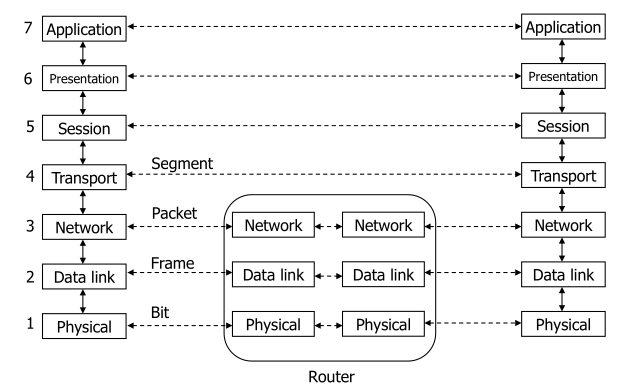
\includegraphics[width=0.4\textwidth]{./images/osi_router.png}
%   \caption{OSI Router}
%   \label{fig:osi_router}
% \end{figure}
%
% Da notare che se il router ha la parte di network separate, allora i due lati edllo strato network hanno protocolli diversi e il router deve fare da nterprete.
%
%
% \subsection{ISO/OSI Layers: Functions in Detail}
%
% \begin{itemize}
%   \item \textbf{Layer fisico}: trasmissione dei bit
%   \item \textbf{Layer data link}: trasmissione dei frame
%   \item \textbf{Layer network}: trasmette dei pacchetti
%   \item \textbf{Layer transport}: trasmissione sicura dei frammenti
%   \item \textbf{Layer session}: gestione della sessione
%   \item \textbf{Layer presentation}: definisce sintassi e semantica dell'informazione
%   \item \textbf{Layer application}: comunicazione fra applicazioni
% \end{itemize}



\subsection{Perchè usare i bus?}
Un bus che collega tutti i componenti al posto di avere una topologia a grafo completo ha i seguenti vantaggi:
\begin{itemize}
  \item \textbf{Riduzione dei costi}: meno cavi e meno connettori
  \item \textbf{Riduzione del peso}: meno cavi
  \item \textbf{Riduzione del volume}: meno cavi
  \item \textbf{Alta modularità}: modifica veicoli
  \item \textbf{Alta modularità}: cooperazione con OEM
  \item \textbf{Modularità}: riuso di moduli
  \item \textbf{Standardizzazione}: standardizzazione dei componenti e dei protocolli (meno errori scemi)
\end{itemize}





